\documentclass{beamer}

\usepackage[utf8]{inputenc}
\usepackage[T1]{fontenc}
\usepackage{lmodern}
\usepackage{graphicx}
\usepackage{amsmath}
\usepackage[french]{babel}
\usepackage{array}

\mode<presentation> {
  \usetheme{Madrid}
  \setbeamertemplate{navigation symbols}{}
}

\title[Analyse de iSudoku]{Analyse de iSudoku}
\subtitle[\ldots]{Projet de l'UE Ingénierie du Logiciel}
\author{
  Maude \bsc{Bellamy}
  \and
  Antoine \bsc{Houssais}
  \and
  Théo \bsc{Lebourg}
  \and
  Jérôme \bsc{Rahault}
  \and
  Fabricio \bsc{Santolin Da Silva}
  \and
  Simon \bsc{Tchernia}
}
\institute[UPMC]{Université Pierre et Marie Curie}
\date{\today}

\AtBeginSection[] {
  \begin{frame}
    \frametitle{Sommaire}
    \tableofcontents[currentsection, hideothersubsections, pausesubsections]
  \end{frame}
}

\begin{document}

\maketitle

\section{Phase de conception}
\subsection {Diagramme de composant et interfaces requises/offertes}
\begin{frame}
  \frametitle{Notre diagramme de composant et leurs interfaces requises/offerts}
  \begin{figure}[h]
    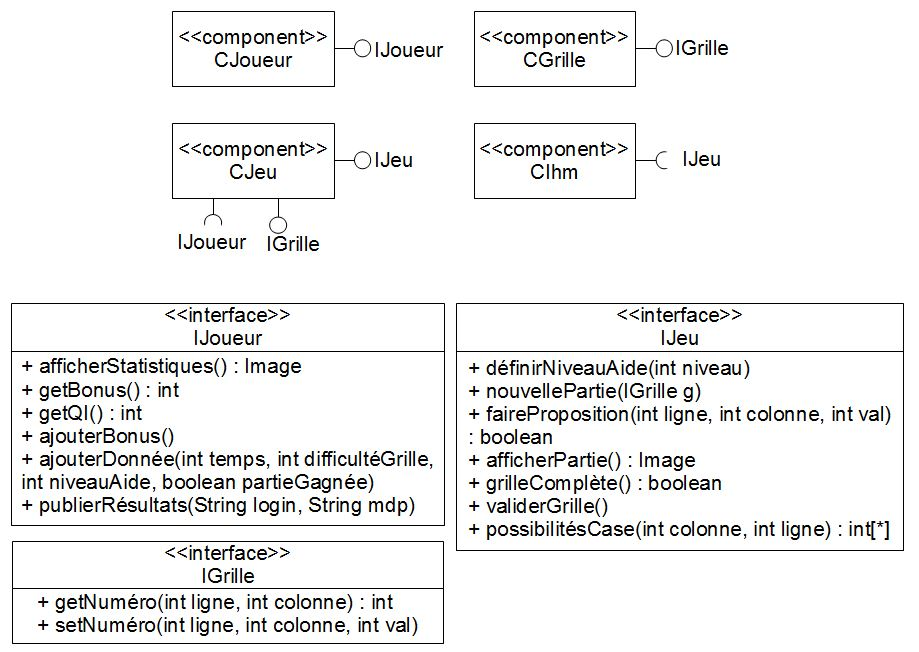
\includegraphics[scale=0.5]{diagramme_composants.JPG}
  \end{figure}
\end{frame}

\subsection{Quelques diagrammes de séquence de niveau interaction inter-composant}
\begin{frame}
  \frametitle{Diagramme de séquence « Jouer une partie »}
  \begin{figure}[h]
    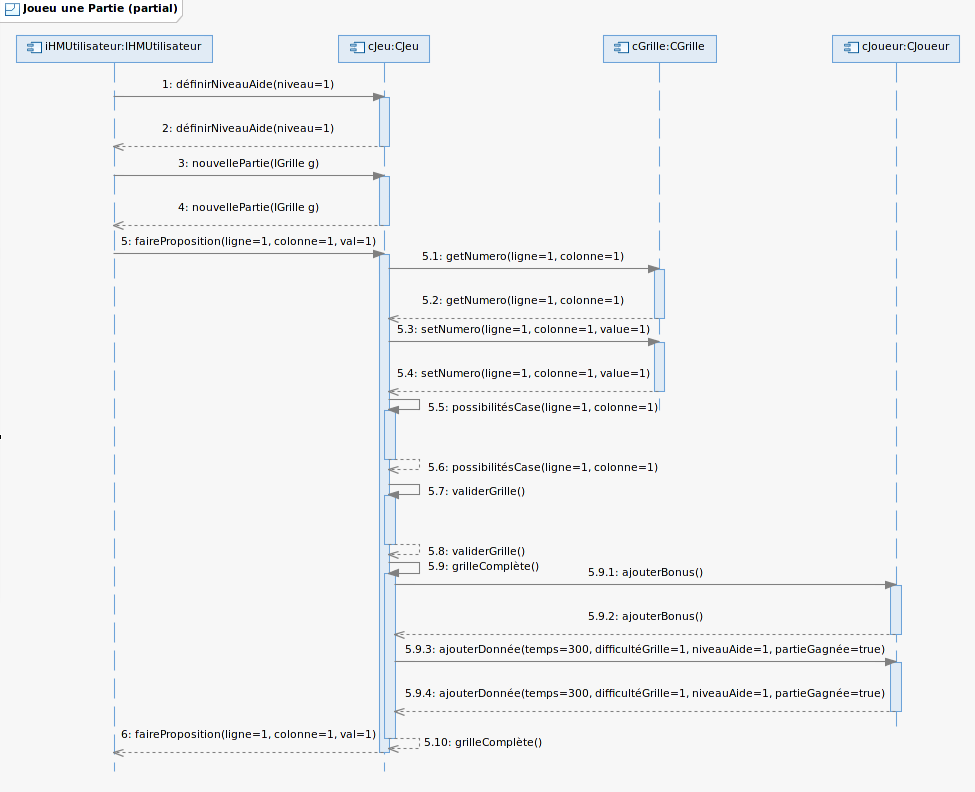
\includegraphics[scale=0.275]{diagrammeSequence_01.png}
  \end{figure}
\end{frame}

\begin{frame}
  \frametitle{Diagramme de séquence « Affiche statistiques »}
  \begin{figure}[h]
    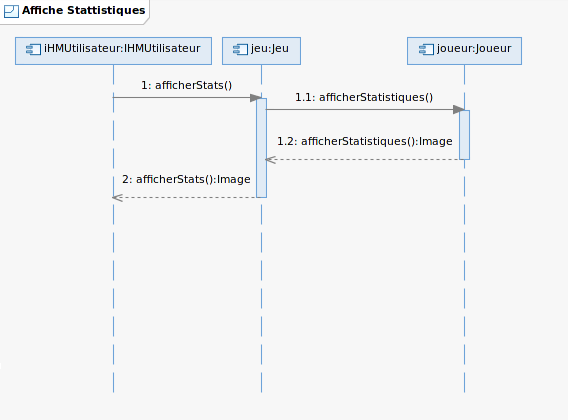
\includegraphics[scale=0.275]{diagrammeSequence_02.png}
  \end{figure}
\end{frame}

\begin{frame}
  \frametitle{Diagramme de séquence « Générer une grille par photo »}
  \begin{figure}[h]
    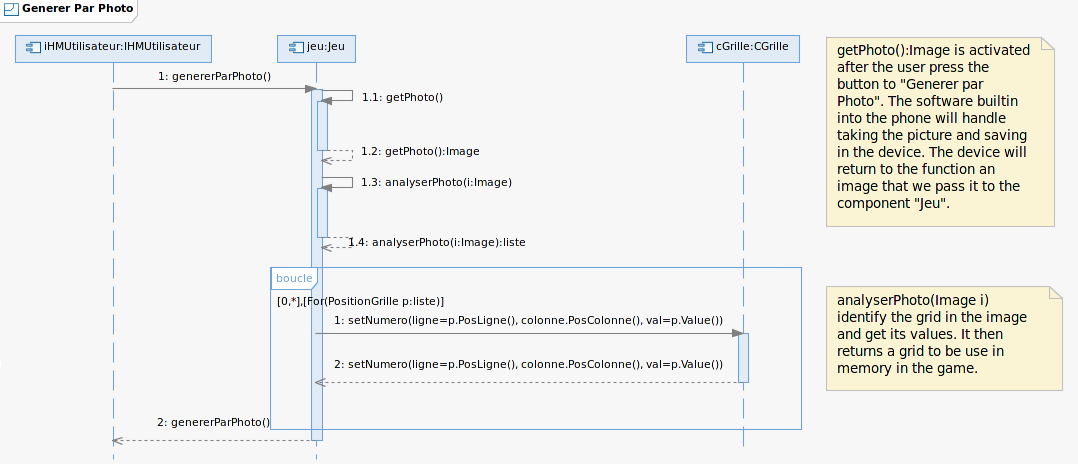
\includegraphics[scale=0.3]{diagrammeSequence_03.png}
  \end{figure}
\end{frame}


\subsection{Instanciation nominale des composants}
\begin{frame}
\frametitle{Instanciation nominale des composants}
  \begin{figure}[h]
    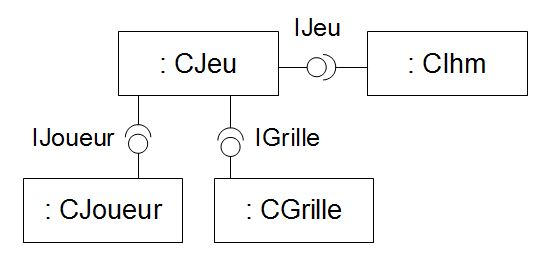
\includegraphics[scale=0.6]{diagramme_instanciation_nominale.JPG}
  \end{figure}
\end{frame}

\subsection{Diagrammes de classe de niveau conception détaillée}

\begin{frame}
\frametitle{Diagramme de classe de niveau conception détaillée}
  \setbeamertemplate{blocks}[default]
  \begin{block}{\footnotesize{CGrille}}
    \begin{figure}[h]
      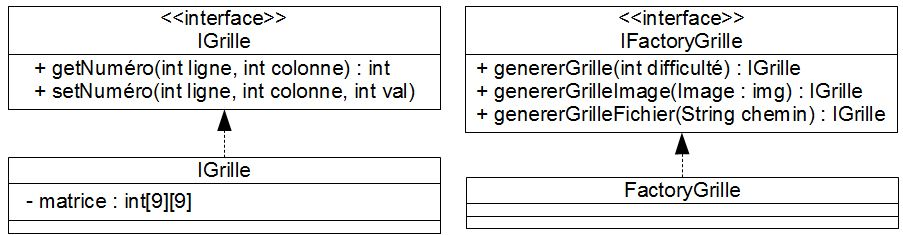
\includegraphics[scale=0.37]{diagramme_classe_detaillee_CGrille.JPG}
    \end{figure}
  \end{block}
  \pause
  \begin{block}{\footnotesize{CJeu}}
    \begin{figure}[h]
      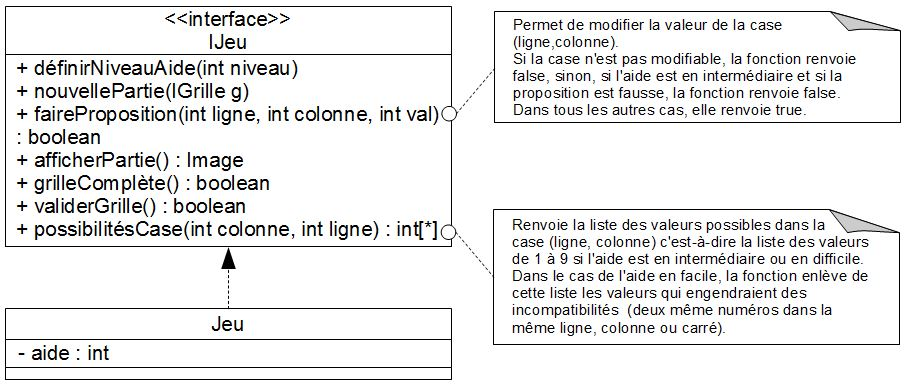
\includegraphics[scale=0.37]{diagramme_classe_detaillee_CJeu.JPG}
    \end{figure}
  \end{block}
\end{frame}

\begin{frame}
\frametitle{Diagramme de classe de niveau conception détaillée}
 \setbeamertemplate{blocks}[default]
  \begin{block}{\footnotesize{CJoueur}}
    \begin{figure}[h]
      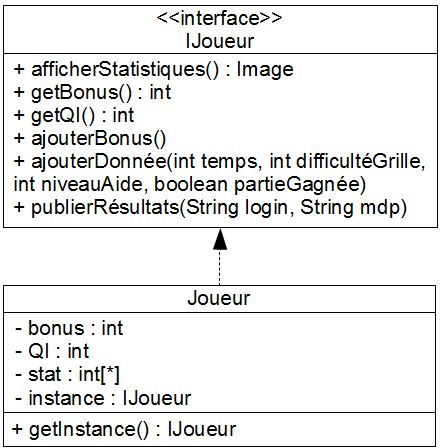
\includegraphics[scale=0.37]{diagramme_classe_detaillee_CJoueur.JPG}
    \end{figure}
  \end{block}
\end{frame}

\subsection{Tests d’intégration}
\begin{frame}
  \frametitle{Test d’intégration \no 1 du cas d'utilisation « Jouer une valeur en difficulté facile »}
  \setbeamertemplate{blocks}[default]
  \begin{block}{\footnotesize{Titre}}
    \scriptsize{Terminer une partie en jouant une valeur correcte en niveau facile}
  \end{block}
  \pause
  \begin{block}{\footnotesize{Contexte}}
    \scriptsize{Une partie a été lancée en niveau « facile » (cf. Test \no x) et il reste une case à complèter}
  \end{block}
  \begin{block}{\footnotesize{Scénario}}
    \begin{enumerate}
      \setbeamertemplate{enumerate item}[circle]
      \item
        \scriptsize{L’utilisateur clique sur la case à remplir}
      \item
        \scriptsize{Le système affiche la valeur possible}
      \item
        \scriptsize{L’utilisateur entre la valeur correcte}
      \item
        \scriptsize{Le système valide la grille et affiche les statistiques de la partie}
    \end{enumerate}
  \end{block}
  \pause
  \begin{block}{\footnotesize{Résultat attendu}}
    \scriptsize{Le partie est terminée.}
  \end{block}
  \begin{block}{\footnotesize{Moyen de vérification}}
    \scriptsize{Visuelle : un message annonçant que la grille a été correctement complétée est affiché}
  \end{block}
\end{frame}
\begin{frame}
  \frametitle{Test d’intégration \no 2 du cas d'utilisation « Générer une grille via une photo »}
  \setbeamertemplate{blocks}[default]
  \begin{block}{\footnotesize{Titre}}
    \scriptsize{Générer une grille de iSudoku en prenant une photo}
  \end{block}
  \pause
  \begin{block}{\footnotesize{Scénario}}
    \begin{enumerate}
      \setbeamertemplate{enumerate item}[circle]
      \item
        \scriptsize{L’utilisateur clique sur le bouton « prendre une photo »}
      \item
        \scriptsize{L’utilisateur prend une photo d’une grille de Sudoku}
      \item
        \scriptsize{Le système affiche que la grille a bien été générée}
      \item
        \scriptsize{Le système affiche la grille} 
    \end{enumerate}
  \end{block}
  \pause
  \begin{block}{\footnotesize{Résultat attendu}}
    \scriptsize{La grille « numérisée » est identique à celle prise en photo.}
  \end{block}
  \begin{block}{\footnotesize{Moyen de vérification}}
    \scriptsize{Visuelle : la grille apparait sur l’application et est prête à être remplie}
  \end{block}
\end{frame}

\section{Génération de code}

\begin{frame}
\frametitle{Diagramme de classe}
  \begin{figure}[h]
      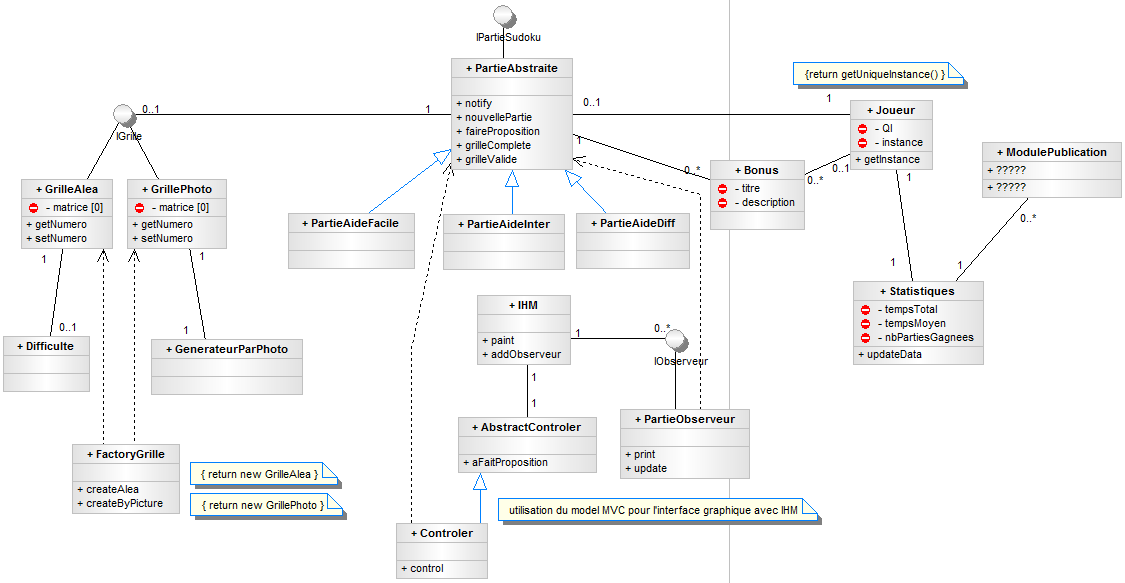
\includegraphics[scale=0.4]{DiagrammeClasseGenere.png}
    \end{figure}
\end{frame}
\end{document}
